
% Aufwandschätzung, Zeitplan, Projektplan
\section{Projektmanagement}
\label{sec:Projektmanagement}

\subsection{Vorgehen}
\label{sub:Vorgehen}

Für die Studienarbeit wurde das agile Vorgehen SCRUM in Kombination mit \acs{RUP} gewählt. Grund für diese Entscheidung ist, dass das agile Vorgehen der noch zu Beginn unklaren Aufgabenstellung entgegenkommt, welche dann iterativ erarbeitet werden konnte. Die wöchentlichen Besprechungen und Reviews mit dem Betreuer ist ein weiterer Grund für diese Entscheidung. Die Kombination mit \acs{RUP} ermöglicht es, dass Projekt in einzelne Phasen aufzuteilen, um so das Ziel und die Zeit nicht aus den Augen zu verlieren.

\subsubsection{Entwicklung}
\label{sub:Entwicklung}

Der Source-Code, wie auch diese Arbeit wird mit Git verwaltet und ist auf Github abgelegt. Die Entwicklung und das Dokumentieren erfolgt nach dem Github-Flow. Der Master-Branch ist auf allen Repositories während der ganzen Zeit gesperrt, so dass er nur über Pull-Requests bearbeitet werden kann. Für jede User-Story wird ein Branch erstellt. Ist die User-Story implementiert, wird ein Pull-Request erstellt und dem anderen Projekt-Mitglied zum Review übergeben. Wird der Pull-Request akzeptiert, wird der Feature-Branch in den Master gemerged. Dieses Vorgehen hat den Vorteil, dass alle Änderungen, welche in den Master gelangen, ein Review durchlaufen müssen und so die Qualität hochgehalten werden kann.


\subsection{Zeitplanung}
\label{sub:Zeitplanung}

Die Arbeitspakte und Zeit wird mithilfe von Jira verwaltet. Für alle Tätigkeiten werden User Stories im Backlog erfasst, priorisiert und geschätzt. Die Schätzung der User Stories erfolgte mit Story Points. Die Arbeitszeitverbuchung wurde auf User Story-Stufe mit Stunden gemacht. 

\subsubsection{Phasen / Iterationen und Meilensteine}
\label{sub:Phasen / Iterationen und Meilensteine}

Die Studienarbeit wird in die \ac{RUP}-Phasen (Inception, Elaboration, Construction, Transition) aufgeteilt. Dabei wird jedoch eine von der gängigen Norm abweichende Aufteilung gewählt. Durch den theoretischen Fokus der Arbeit wird der Elaboration das grösste Zeitbudget zugeordnet. Dies ist auch der Grund warum mit einwöchigen Sprints gearbeitet wird. Es wird zusätzlich vom Standard-\ac{RUP}-Prozess abgewichen. Gegen Ende des Projekts wird nochmals eine zusätzliche Elaboration-Phase durchgeführt. Dieser theoretischer Teil wird nicht in der ersten Elaboration gemacht, damit der wichtigste Use Case \textit{Fussgänger-Routing über offene Flächen} so sicher umgesetzt wird und gegen Ende des Projekts bei idealem Projektverlauf noch Zeit für die Aufbereitung von \textit{Stand Fussgänger-Routing über offene Strassen} und \textit{Stand Flächen-Traversierung über Berge/Strände} bleibt.

\begin{landscape}
\begin{longtable}{l p{5.5cm} p{5.5cm} p{5.5cm}} 
        \toprule
        \textbf{Sprint}
                                & \textbf{Sprint 0}
                                & \textbf{Sprint 1}
                                & \textbf{Sprint 2} \\
        
        \midrule
        \textbf{Phase}
                                & Inception
                                & Inception
                                & Elaboration \\
        
        \textbf{Milestones} 	
                                & \textit{Aufgabenstellung}
                                & \textit{Aufgabenstellung}
                                & \textit{Stand Fussgänger-Routing über offene Flächen}  \\
        
        \textbf{Arbeitspakete}
                                & \begin{enumerate}[noitemsep]
                                    \item Aufgabestellung-Brainstorming
                                    \item JIRA aufsetzen
                                    \item LATEX Doc aufsetzen
                                    \item Vorgehen definieren
                                \end{enumerate}
                                & \begin{enumerate}[noitemsep]
                                    \item Aufgabenstellung finalisieren
                                    \item Travis aufsetzen
                                    \item Python/Docker Know-How aufbauen
                                    \item Einarbeitung QGIS
                                \end{enumerate}
                                & \begin{enumerate}[noitemsep]
                                    \item Visibility-Graph Know-How sammeln
                                    \item Visibility-Graph QGIS Test
                                    \item SpiderWeb-Graph Know-How sammeln
                                \end{enumerate}  \\
        
        \pagebreak
        \toprule
        \textbf{Sprint}
                                & \textbf{Sprint 3}
                                & \textbf{Sprint 4}
                                & \textbf{Sprint 5} \\
        
        \midrule
        \textbf{Phase}
                                & Elaboration
                                & Elaboration
                                & Elaboration \\
        
        \textbf{Milestones}
                                & \textit{Stand Fussgänger-Routing über offene Flächen}
                                & \textit{Backend Prototype}
                                & \textit{Backend Prototype}  \\
        
        \textbf{Arbeitspakete}
                                & \begin{enumerate}[noitemsep]
                                    \item Visibility-Graph QGIS Test
                                    \item SpiderWeb-Graph QGIS Test
                                    \item Skeleton-Graph Know-How sammeln
                                \end{enumerate}
                                & \begin{enumerate}[noitemsep]
                                    \item Evaluation Routing Engines
                                    \item Evaluation Overpass Anbindung
                                    \item Konzept Platz-Vorverarbeitung erstellen
                                \end{enumerate}
                                & \begin{enumerate}[noitemsep]
                                    \item Architektur Backend
                                    \item Evaluation Search.ch Anbindung
                                    \item Platz-Vorverarbeitung umsetzen
                                \end{enumerate}  \\
        
        
        \toprule
        \textbf{Sprint}
                                & \textbf{Sprint 6}
                                & \textbf{Sprint 7}
                                & \textbf{Sprint 8} \\
        
        \midrule
        \textbf{Phase}
                                & Construction
                                & Construction
                                & Construction \\
        
        \textbf{Milestones}
                                & \textit{Backend Prototype}
                                & \textit{Backend Prototype}
                                & \textit{Backend/Frontend Prototype}  \\
        
        \textbf{Arbeitspakete}
                                & \begin{enumerate}[noitemsep]
                                    \item Anbindung Fremdsysteme
                                    \item Platz-Vorverarbeitung umsetzen
                                    \item API definieren
                                \end{enumerate}
                                & \begin{enumerate}[noitemsep]
                                    \item Kommunikation mit Fremdsystemen koordinieren
                                    \item QGIS-Plugin Grundstruktur
                                \end{enumerate}
                                & \begin{enumerate}[noitemsep]
                                    \item Vergleich Flächentraversierungsvarianten durchführen
                                    \item QGIS-Plugin Eingabemaske
                                    \item Stand Start-/Endpunkt auf Flächen
                                \end{enumerate} \\
        
        
        \pagebreak
        \toprule
        \textbf{Sprint}
                                & \textbf{Sprint 9}
                                & \textbf{Sprint 10}
                                & \textbf{Sprint 11} \\
        
        \midrule
        \textbf{Phase}
                                & Construction
                                & Elaboration
                                & Elaboration \\
        
        \textbf{Milestones}
                                & \textit{Prototyp Frontend}
                                & \textit{Stand Fussgänger-Routing über offene Strassen}
                                & \textit{Stand Flächen-Traversierung über Berge/Strände}  \\
        
        \textbf{Arbeitspakete}
                                & \begin{enumerate}[noitemsep]
                                    \item QGIS-Plugin beste Route anzeigen
                                    \item Stand Flächentraversierung bei zwei benachbarten Polygonen

                                \end{enumerate}
                                & \begin{enumerate}[noitemsep]
                                    \item Stand Fussgänger-Routing über offene Strassen Recherche
                                    \item Überführung in Docker-Container
                                \end{enumerate}
                                & \begin{enumerate}[noitemsep]
                                    \item Stand Flächen-Traversierung über Berge/Strände Recherche
                                \end{enumerate} \\
                                
        
        \toprule
        \textbf{Sprint}
                                & \textbf{Sprint 12}
                                & \textbf{Sprint 13}
                                & \\
        
        \midrule
        \textbf{Phase}
                                & Transition
                                & Transition
                                & \\
        
        \textbf{Milestones}
                                & \textit{Abgabe SA}
                                & \textit{Abgabe SA}
                                & \\
        
        \textbf{Arbeitspakete}
                                & \begin{enumerate}[noitemsep]
                                    \item Restarbeiten
                                    \item Doku aufräumen
                                    \item Abgabe vorbereiten
                                \end{enumerate}
                                & \begin{enumerate}[noitemsep]
                                    \item Abgabe SA
                                \end{enumerate}
                                & \\
        
        \bottomrule
    \caption{Phasen / Iterationen und Meilensteine}
    \label{table:Phasen / Iterationen und Meilensteine}
\end{longtable}
\end{landscape}

\subsection{Risiken}
\label{sub:Risiken}

\begin{table}[ht]
    \centering
    \caption{Risiken}
    \label{Risiken}
    \begin{tabular}{lllll}
        \textbf{ID} & \textbf{Risiko}                                                                                    & \textbf{\begin{tabular}[c]{@{}l@{}}max.\\ Schaden {[}h{]}\end{tabular}} & \textbf{WSK} & \textbf{\begin{tabular}[c]{@{}l@{}}gewichteter\\ Schaden\end{tabular}} \\
        1           & \begin{tabular}[c]{@{}l@{}}nicht-existentielle Flächenverarbeitungs-\\ algorithmen\end{tabular}    & 32                                                                      & 40\%         & 12.8                                                                   \\
        2           & \begin{tabular}[c]{@{}l@{}}Schwierigkeiten mit der Implementation \\ der Algorithmen\end{tabular}  & 16                                                                      & 20\%         & 3.2                                                                    \\
        3           & \begin{tabular}[c]{@{}l@{}}Technologie eignet sich nicht für \\ die Vorverarbeitung\end{tabular}   & 32                                                                      & 20\%         & 6.4                                                                    \\
        4           & viele Abhängigkeiten auf Fremdsysteme                                                              & 8                                                                       & 20\%         & 1.6                                                                    \\
        5           & \begin{tabular}[c]{@{}l@{}}Fremdsysteme bieten nicht die \\ geforderte Funktionalität\end{tabular} & 32                                                                      & 30\%         & 9.6                                                                    \\
        6           & Scope zu gross angesetzt                                                                           & 24                                                                      & 30\%         & 7.2                                                                   
    \end{tabular}
\end{table}

Das Hauptrisiko der Arbeit ist der grosse theoretische Aspekt, welcher viele Unbekannten bieter. So ist nicht klar, ob der aktuelle Stand der Technik genügend Material als Grundlage liefert, um das Problem der Traversierung von Flächen zu beheben. Auch ist nicht bekannt, ob sich Python als Technologie eignet, um grosse Mengen an \ac{OSM}-Daten zu verarbeiten. Die Arbeit mit Fremdsystemen birgt in vieler Hinsicht Risiken. Ob die Fremdsysteme die gewünschten Funktionalität in dem Umfang liefert, welcher benötigt wird, muss zuerst abgeklärt werden. Das eine Routing-Engine beispielsweise problemlos auf den von uns vorverarbeitenden \ac{OSM} operieren kann, muss zwingend schnellstmöglich sichergestellt werden, da dies massgeblich verantwortlich für den Erfolg der Arbeit ist.

\begin{figure}[ht]
    \centering
    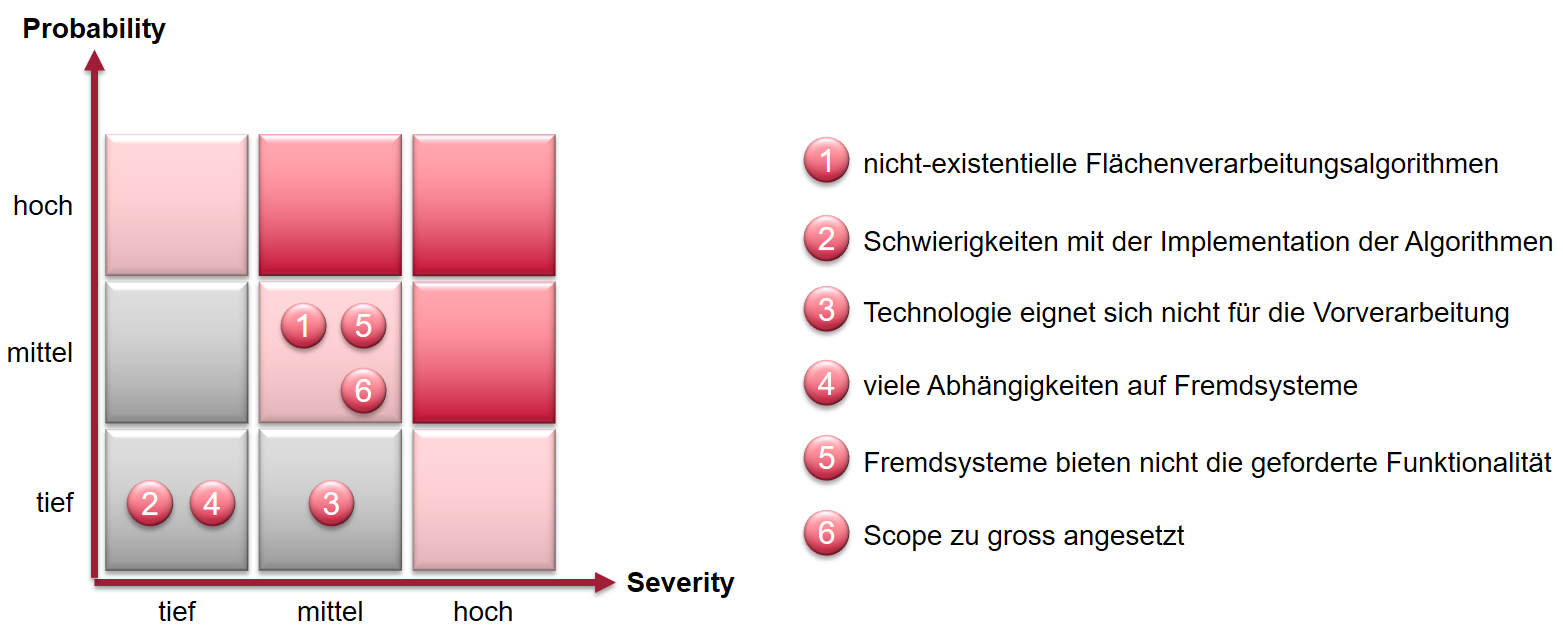
\includegraphics[width=1\linewidth]{projectdoc/img/risk_analysis}
    \caption[Risiko Analyse]{Risiko Analyse}
    \label{fig:risk_analysis}
\end{figure}

\subsubsection{Umgang mit Risiken}
\label{Risiken:Umang mit Risiken}
Um dem Hauptrisiko des Projekts, sprich die Evaluation, Optimierung und Implementation der Flächenverarbeitungsalgorithmen entgegen zu wirken, ist die Elaboration-Phase 4 Sprints lang und die Umsetzung der Algorithmen zu Beginn der Construction-Phase angesiedelt, um so genügend Spielraum zu haben. Treten in der Elaboration-Phase Probleme mit diesem Punkt auf oder man sieht, dass sich Python für diesen Zweck nicht eignet, muss dementsprechend der Scope des Frontends (QGIS Plugin) gekürzt werden. Dies aus dem einfachen Grund, da ohne diese Grundlage auch keine Visualisierung Sinn macht. Nach der Elaboration ist auch bekannt, ob alle Fremdsysteme die Anforderungen erfüllen. Ist dies nicht der Fall, können bei search.ch \cite{search_ch_route_api} Change-Requests beantragt werden. Je nach Priorisierung dieser durch search.ch muss der Zeitplan aktualisiert und der Scope gekürzt werden. Kann die Routing-Engine auf den vorverarbeitenden \ac{OSM}-Daten nicht operieren, so muss weiteren Aufwand in Anpassung der Verarbeitung der \ac{OSM}-Daten gesteckt werden, was ebenfalls eine Kürzung des Scopes zur Folge hat.

\subsubsection{Konsequenz}
\label{Risiken:Konsequenz}
Tritt eines der Hauptrisiken (WSK > 9) ein, muss der Prototyp (QGIS-Plugin) aus dem Scope gestrichen werden. Die kleineren Risiken vermindern die Funktionsweise des Prototyps.

\subsection{Team, Rollen und Verantwortlichkeiten}
\label{sub:Team, Rollen und Verantwortlichkeiten}

\begin{table}[H]
    \centering
    \caption{Team, Rollen und Verantwortlichkeiten}
    \label{table: Team, Rollen und Verantwortlichkeiten}
    \begin{tabular}{lll}
        & \textbf{Rolle} & \textbf{Verantwortlichkeiten}    \\
        Prof. Stefan Keller  &        Betreuer                   &    \\
        Robin Suter          &        Autor                      & Plaza Preprocessing \\
        Jonas Matter         &        Autor                      & PlazaRouting Backend, QGIS-Plugin
    \end{tabular}
\end{table}